\phantomsection
\chapter{Analisi dei cluster}\label{cap5}

L'analisi dei cluster è una metodologia che permette di raggruppare in più sottoinsiemi, detti \textit{cluster}, entità (unità) appartenenti a un insieme più ampio. Sia $I = I_1, I_2, ..., I_n$ un insieme di \textit{n} individui (entità o unità) appartenenti a una popolazione ideale. Si assuma che esista un insieme di caratteristiche $C = C_1, C_2, ..., C_p$ che sono osservabili e sono possedute da ogni individuo in \textit{I}. Il termine osservabile denota caratteristiche che danno origine a dati sia di tipo qualitativo che di tipo quantitativo (detti anche misure).

In generale, quello che viene fatto è porre una matrice X, di cardinalità \textit{np}, gli individui \textit{I} e le misure \textit{C}; gli $x_{ij}$ denotano il valore della misura della caratteristica j-esima relativa all'individuo $I_i$.

Il problema dell'analisi dei cluster consiste nel determinare \textit{m} sottoinsiemi, detti cluster, di individui in \textit{I}, con \textit{m} intero minore di \textit{n}, tali che $I_i$ appartenga soltanto a un unico sottoinsieme. Gli individui che sono assegnati allo stesso cluster sono detti simili mentre gli individui che sono assegnati a differenti cluster sono detti dissimili.

Lo scopo è distribuire le osservazioni in gruppi in modo tale che il grado di naturale associazione sia alto tra i membri dello stesso gruppo e basso tra i membri di gruppi diversi. In questo modo si otterrà quindi un'alta omogeneità all'interno dei gruppi e un'alta eterogeneità tra gruppi distinti.

In questo capitolo, per l'analisi e la suddivisione in cluster verranno analizzati i seguenti metodi di raggruppamento:

\begin{itemize}
    \item Metodi Gerarchici:
    \begin{itemize}
        \item Metodo del legame singolo;
        \item Metodo del legame completo;
        \item Metodo del legame medio;
        \item Metodo del centroide;
        \item Metodo della mediana;
    \end{itemize}
    \item Metodi non Gerarchici (partizionali):
    \begin{itemize}
        \item Metodo del k-means;
    \end{itemize}
\end{itemize}

Questi metodi hanno lo scopo di trovare una partizione ottima degli individui del dataset, in modo da dividerli equamente in cluster. Al fine di operare su dati uguali, non considerando l'unità di misura, si raccomanda la standardizzazione di ogni variabile (caratteristica) usando la media campionaria e la deviazione standard campionaria, entrambe derivate dall'insieme completo di individui della popolazione.

\vspace{5mm}
\begin{lstlisting}
  df_scaled <- scale(df)
  df_scaled
\end{lstlisting}
\vspace{5mm}


\vspace{5mm}
\begin{lstlisting}

                      Modo.Cont.  Modo.Salt. Qualche.Att. Non.Prat.Sport.
Piemonte              0.37410684  0.50417102 -0.078865135    -0.287349873
ValleDAosta           1.38101966  1.22728483  0.486138814    -1.180578217
Liguria              -0.07513119  0.86572792  1.592604881    -0.708683997
Lombardia             0.68392617  0.82555493  1.074684594    -0.927777742
TrentinoAltoAdige     2.51186021  1.38797679  0.085927684    -1.694605849
Veneto                0.65294424  1.38797679  0.603847970    -0.860364282
Friuli-VeneziaGiulia  0.09526944  0.98624689  1.310102906    -0.725537362
Emilia-Romagna        0.68392617  0.02209514  0.556764308    -0.573857078
Toscana               0.45156167  0.62468999  0.509680646    -0.573857078
Umbria                0.01781461 -0.09842382  0.274262334    -0.085109493
Marche                0.29665201 -0.09842382  0.321345996    -0.262069825
Lazio                 0.34312491 -0.45998073 -0.008239641    -0.085109493
Abruzzo              -0.01316732  0.34347906 -0.196574291     0.007584014
Molise               -1.26793560 -1.10274856 -0.384908940     1.060919325
Campania             -1.43833624 -1.78568938 -1.303040357     1.617080370
Puglia               -0.88066144 -0.13859681 -1.750335150     1.145186150
Basilicata           -1.17498981 -0.90188361 -1.538458669     1.381133260
Calabria             -1.20597174 -1.70534340 -0.926371058     1.355853213
Sicilia              -1.23695367 -1.34378650 -1.703251487     1.566520275
Sardegna             -0.19905892 -0.54032671  1.074684594    -0.169376318
attr(,"scaled:center")
     Modo.Cont.      Modo.Salt.    Qualche.Att. Non.Prat.Sport. 
         23.585          10.945          31.835          33.610 
attr(,"scaled:scale")
     Modo.Cont.      Modo.Salt.    Qualche.Att. Non.Prat.Sport. 
       6.455375        2.489235        4.247758       11.867066 

\end{lstlisting}
\vspace{5mm}

Prima di procedere con il calcolo dei cluster con i vari metodi indicati si deve introdurre il concetto di distanza, fondamentale per l'analisi dei cluster.

\section{Distanza}\label{cap5.1}

Per risolvere il problema di clustering è chiaramente desiderabile definire i termini \textit{somiglianza} o \textit{differenza} in modo quantitativo, ossia occorre precisare cosa significa la somiglianza di due individui $I_i$ e $I_j$ assegnati allo stesso cluster e la differenza di due individui assegnati a differenti cluster.

La somiglianza può essere definita mediante una misura di distanza $d_{ij} = d(X_i, X_j)$ tra due individui $I_i$ e $I_j$ (i = j). Le misure di distanza possono assumere qualsiasi valore reale maggiore o uguale a zero. Un criterio per risolvere il problema di clustering potrebbe essere quello di assegnare due individui $I_i$ e $I_j$ allo stesso cluster se la distanza tra i punti $X_i$ e $X_j$ è sufficientemente piccola e a differenti cluster se la distanza tra i punti è sufficientemente grande.

\noindent \textbf{Definizione:} Dato uno spazio Euclideo $E_p$ a $p$ dimensioni, una funzione a valori reali $d(X_i, X_j)$ è detta \textit{funzione distanza} se e soltanto se essa soddisfa le seguenti condizioni:

\begin{enumerate}
    \item $d(X_i, X_j) = 0$ se e solo se $X_i = X_j$, con $X_i$ e $X_j$ in $E_p$;
    \item $d(X_i, X_j) \geq 0$ per ogni $X_i$ e $X_j$ in $E_p$;
    \item $d(X_i, X_j) = d(X_j, X_i)$ per ogni $X_i$ e $X_j$ in $E_p$;
    \item $d(X_i, X_j) \leq d(X_i, X_k) + d(X_k, X_j)$ per ogni $X_i, X_j$ e $X_k$ in $E_p$;
\end{enumerate}

La misura di distanza che viene utilizzata in questo studio è la metrica Euclidea, così definita:

\[d_2 (X_i, X_j) = \left[ \sum_{k=1}^p (x_{ik} - x_{jk})^2\right]^{1/2}  \]

dove $x_{ik}$ è il valore della k-esima caratteristica dell'individuo $I_i$.

In R utilizzando la funzione \textit{dist()} e passando il parametro "euclidean" si può calcolare la matrice delle distanza per il dataset scalato attraverso la metrica euclidea:

\vspace{5mm}
\begin{lstlisting}
dist_e <- dist(df_scaled, method = "euclidean", diag = TRUE, upper = TRUE)
\end{lstlisting}
\vspace{5mm}

Il parametro \textit{method} indica la metrica da utilizzare, \textit{diag = TRUE} indica di mostrare la diagonale della matrice e \textit{upper = TRUE} indica di mostrare la parte superiore della matrice, che è speculare alla parte inferiore. Si presenta così una parte della matrice delle distanze:

\vspace{5mm}
\begin{lstlisting}
                      Piemonte ValleDAosta   Liguria Lombardia
Piemonte             0.0000000    1.6290652 1.8176558 1.3928749
ValleDAosta          1.6290652    0.0000000 1.9230315 1.0284068
Liguria              1.8176558    1.9230315 0.0000000 0.9455292
Lombardia            1.3928749    1.0284068 0.9455292 0.0000000
\end{lstlisting}
\vspace{5mm}

Come è possibile notare, sulla diagonale è sempre presente il valore 0, confermando dunque che la distanza di una regione con se stessa è nulla.

\section{Metodi non gerarchici}\label{cap5.3}

L'obiettivo dei metodi non gerarchici è quello di ottenere un'unica partizione degli n individui di partenza in cluster. A differenza dei metodi gerarchici, in tali tecniche è consentito riallocare gli individui già classificati a un livello precedente dell'analisi. 

Gli algoritmi di tipo non gerarchico procedono, data una prima partizione, a riallocare gli individui nel gruppo con centroide più vicino, fino a che per nessun individuo si verifica che sia minima la distanza rispetto al centroide di un gruppo diverso da quello a cui esso appartiene.

Il metodo più utilizzato prende il nome di \textit{k-means}. Tale metodo richiede che il numero di cluster sia specificato a priori e fornisce in output un'unica partizione.

L'algoritmo è il seguente:

\begin{itemize}
    \item Step 1: Fissare a priori il numero k di cluster specificando m punti di riferimento iniziali che inducono una prima partizione provvisoria;
    \item Step 2: Considerare tutti gli individui e attribuire ciascuno di essi al cluster individuato dal punto di riferimento da cui ha distanza minore;
    \item Step 3: Calcolare il centroide di ognuno dei k gruppi così ottenuti. Tali centroidi costituiscono i punti di riferimento per i nuovi cluster;
    \item Step 4: Valutare la distanza di ogni unità da ogni centroide ottenuto al passo precedente. Se la distanza minima non è ottenuta in corrispondenza del centroide del gruppo di appartenenza, allora si procede a spostare l'individuo presso il cluster che ha il centroide più vicino;
    \item Step 5: Ricalcolare i centroidi dei k gruppi così ottenuti;
    \item Step 6: Ripetere il procedimento a partire dal punto 4 fino a che i centroidi non subiscono ulteriori modifiche rispetto all'iterazione precedente. Si procede così iterativamente a spostamenti successivi fino a che gli individui all'interno di ogni cluster non cambiano al ripetersi del procedimento.
\end{itemize}

Nel metodo k-means, per garantire la convergenza della procedura iterativa, come misura di distanza tra i vettori delle caratteristiche e i centroidi viene utilizzata la distanza euclidea e, come per il metodo del centroide, si considera la matrice contenente i quadrati delle distanze euclidee.

L'analisi con il metodo k-means si effettua in R mediante la funzione $kmeans(X, centers, iter.max = N, nstart = M$ dove X è la matrice dei dati, $centers$ è il numero dei cluster che si vogliono identificare o un vettore di lunghezza pari al numero di cluster contenente un insieme di centroidi iniziali dei cluster, ottenuti con il metodo gerarchico: ad esempio, $iter.max$ è il massimo numero di iterazioni per messe, $nstart$ fornisce il numero di volte in cui ripetere la procedura di scelta casuale dei punti di riferimento, nel caso in cui centers è un numero.

Per l'applicazione del metodo considereremo tre differenti scelte iniziali dei parametri da passare alla funzione: scelta casuale dei punti di riferimento, ripetizione della procedura di scelta casuale dei punti di riferimento e scelta dei centroidi come punti di riferimento

\subsection{Scelta casuale dei punti di riferimento}\label{cap5.3.1}

Con tale metodo si effettua una suddivisione in 3 cluster del dataset effettuando un'unica scelta casuale dei punti di riferimento con un numero massimo di iterazioni pari a 10. Dall'output ottenuto dalla funzione k-means si può osservare che:

\vspace{5mm}
\begin{lstlisting}
  kmrandom <- kmeans(df_scaled, center = 3, iter.max = 10, nstart =1)
  kmrandom

  K-means clustering with 3 clusters of sizes 6, 6, 8

Cluster means:
  Modo.Cont.  Modo.Salt. Qualche.Att. Non.Prat.Sport.
1 -1.2008081 -1.16300804   -1.2677276       1.3544488
2  0.8749814  1.11346136    0.8588845      -1.0162579
3  0.2443700  0.03716002    0.3066324      -0.2536431

Clustering vector:
            Piemonte         ValleDAosta              Liguria 
                   3                    2                    2 
           Lombardia    TrentinoAltoAdige               Veneto 
                   2                    2                    2 
Friuli-VeneziaGiulia       Emilia-Romagna              Toscana 
                   2                    3                    3 
              Umbria               Marche                Lazio 
                   3                    3                    3 
             Abruzzo               Molise             Campania 
                   3                    1                    1 
              Puglia           Basilicata             Calabria 
                   1                    1                    1 
             Sicilia             Sardegna 
                   1                    3 

Within cluster sum of squares by cluster:
[1] 3.638836 7.144400 3.388854
 (between_SS / total_SS =  81.4 %)

 
kmrandom$betweenss
[1] 61.82791
kmrandom$tot.withinss
[1] 14.28099
kmrandom$totss
[1] 76
\end{lstlisting}
\vspace{5mm}

Il metodo k-means individua una partizione in 3 cluster, dove gli individui dei cluster sono indicati in "Clustering vector". I centroidi sono indicati in "Cluster means", infatti il primo cluster ha centroide di coordinate (-1.20, -1.16, -1.27, 1.35). I valori sotto la voce "Within cluster" rappresentano le misure di non omogeneità statistica associate ai cluster (ottenendo $trS = 14.28099$), mentre la misura di non omogeneità totale può essere visionata con $kmrandom\$totss = 76$. Si nota dunque che l'esecuzione del metodo ha portato ad avere una misura di non omogeneità tra i cluster pari a 81.4\% ($\frac{trB}{trT}$), confermando che la clusterizzazione in 3 fornisce ottimi risultati.

\subsection{Ripetizione della scelta casuale dei punti di riferimento}\label{cap5.3.2}

Con tale metodo si effettua una suddivisione in 3 cluster del dataset richiedendo che l'algoritmo di aggregazione venga ripetuto 10 volte in corrispondenza di 10 ripetizioni della procedura di scelta casuale dei punti di riferimento con un massimo di iterazioni pari a 10.

\vspace{5mm}
\begin{lstlisting}
  kmrandom1 <- kmeans(df_scaled, center = 3, iter.max = 10, nstart = 10)
  kmrandom1

K-means clustering with 3 clusters of sizes 6, 6, 8

Cluster means:
  Modo.Cont.  Modo.Salt. Qualche.Att. Non.Prat.Sport.
1  0.8749814  1.11346136    0.8588845      -1.0162579
2 -1.2008081 -1.16300804   -1.2677276       1.3544488
3  0.2443700  0.03716002    0.3066324      -0.2536431

Clustering vector:
            Piemonte         ValleDAosta              Liguria 
                   3                    1                    1 
           Lombardia    TrentinoAltoAdige               Veneto 
                   1                    1                    1 
Friuli-VeneziaGiulia       Emilia-Romagna              Toscana 
                   1                    3                    3 
              Umbria               Marche                Lazio 
                   3                    3                    3 
             Abruzzo               Molise             Campania 
                   3                    2                    2 
              Puglia           Basilicata             Calabria 
                   2                    2                    2 
             Sicilia             Sardegna 
                   2                    3 

Within cluster sum of squares by cluster:
[1] 7.144400 3.638836 3.388854
 (between_SS / total_SS =  81.4 %)  

kmrandom1$betweenss
[1] 61.82791
kmrandom1$tot.withinss
[1] 14.17209
kmrandom1$totss
[1] 76
\end{lstlisting}
\vspace{5mm}

L'esecuzione del metodo in questo caso ha portato ad avere una misura di non omogeneità tra i cluster pari a 81.4\%, confermando che la clusterizzazione in 3 cluster è buona.

\subsection{Scelta dei centroidi come punti di riferimento}\label{cap5.3.3}

\vspace{5mm}
\begin{lstlisting}
  df_scaled <- scale(df)
  dist_e <- dist(df_scaled, method = "euclidean", diag = TRUE, upper = TRUE)
  dist_e2 <- dist_e^2
  cluster_centroid <- clusteringCentroide(df)
  cut_centroid <- cutree(cluster_centroid, k = 3)
  cutList_centroid <- list(cut_centroid)
  initCentroids <- aggregate(df_scaled, cutList_centroid, mean)[, -1]
  initCentroids

  Modo.Cont. Modo.Salt. Qualche.Att. Non.Prat.Sport.
1  0.3609991  0.4300055   0.57849523      -0.4947759
2  2.5118602  1.3879768   0.08592768      -1.6946058
3 -1.2008081 -1.1630080  -1.26772761       1.3544488
\end{lstlisting}
\vspace{5mm}

Utilizzando i centroidi appena calcolati, si può applicare il metodo k-means

\vspace{5mm}
\begin{lstlisting}
  kmcentroid <- kmeans(df_scaled, center = initCentroids, iter.max = 10)
  kmcentroid

K-means clustering with 3 clusters of sizes 11, 3, 6

Cluster means:
  Modo.Cont. Modo.Salt. Qualche.Att. Non.Prat.Sport.
1  0.2417295  0.2704373    0.5845865      -0.3991949
2  1.5152747  1.3344128    0.3919715      -1.2451828
3 -1.2008081 -1.1630080   -1.2677276       1.3544488

Clustering vector:
            Piemonte         ValleDAosta              Liguria 
                   1                    2                    1 
           Lombardia    TrentinoAltoAdige               Veneto 
                   1                    2                    2 
Friuli-VeneziaGiulia       Emilia-Romagna              Toscana 
                   1                    1                    1 
              Umbria               Marche                Lazio 
                   1                    1                    1 
             Abruzzo               Molise             Campania 
                   1                    3                    3 
              Puglia           Basilicata             Calabria 
                   3                    3                    3 
             Sicilia             Sardegna 
                   3                    1 

Within cluster sum of squares by cluster:
[1] 8.368460 2.273698 3.638836
 (between_SS / total_SS =  81.2 %)

kmcentroid$totss
[1] 76
kmcentroid$betweenss
[1] 61.71901
\end{lstlisting}
\vspace{5mm}

In questo caso, la misura di non omogeneità tra i cluster è di pochissimo inferiore a quella ottenuta dai due metodi precedentemente usati, dunque è risultato irrilevante l'impiego dei centroidi.

\section{Metodi gerarchici}\label{cap5.2}

I metodi di clustering gerarchico possono essere di due tipi: \textit{agglomerativi} e \textit{divisivi}. I metodi gerarchici di tipo agglomerativo partono da una situazione in cui si hanno \textit{n} cluster distinti, ognuno contenente un solo individuo, fino a giungere a una situazione dove si ha un solo cluster che contiene tutti gli \textit{n} individui mediante successive unioni dei cluster meno distanti tra loro. Invece, i metodi gerarchici di tipo divisivo partono da una situazione in cui si ha un solo cluster che contiene tutti gli \textit{n} individui per giungere, attraverso successive divisioni dei cluster più distanti tra loro, a una situazione in cui si hanno \textit{n} cluster distinti ognuno contenente un solo individuo.

L'obiettivo dei metodi gerarchici non è quello di ottenere una singola partizione degli \textit{n} individui di partenza ma di ottenere una sequenza di partizioni che possono essere rappresentate graficamente mediante una struttura ad albero, detta \textit{dendrogramma}, nella quale sull'insieme delle ordinate sono riportati i livelli di distanza a cui avviene l'agglomerazione mentre sull'asse delle ascisse sono riportati i singoli individui. Ad ogni livello di distanza corrisponde una partizione. Dunque, il dendrogramma fornisce un quadro completo della struttura dell'insieme in termini delle misure di distanza tra gli individui.

Di seguito, l'algoritmo del dendrogramma:

\begin{itemize}
    \item Step 1: A partire dalla matrice X dei dati o dalla matrice scalata, considerare la matrice delle distanze D tra gli individui considerati come singoli cluster contenenti un solo individuo;
    \item Step 2: Individuare la coppia di cluster meno distanti e raggruppare in un unico cluster i due cluster meno distanti; calcolare in seguito la distanza di questo nuovo cluster rispetto a tutti gli altri gruppi già esistenti;
    \item Step 3: Costruire una nuova matrice di distanza, la quale risulterà ridotta di una riga e di una colonna rispetto a quella precedente;
    \item Step 4: Operare sulla matrice così ottenuta a partire dal passo 2 fino al'esaurimento di tutte le possibilità di raggruppamento;
    \item Step 5: Rappresentare graficamente il processo di agglomerazione attraverso un dendrogramma.
\end{itemize}

I metodi gerarchici che si andranno ad analizzare saranno i metodi agglomerativi.

\subsection{Metodo del legame singolo}\label{cap5.2.1}

In questo metodo, la distanza tra i gruppi $G_1$ (contenente $n_1$ individui) e $G_2$ (contenente $n_2$ individui) è definita come la \textit{minima} tra tutte le $n_1 n_2$ distanze che si possono calcolare tra ogni individuo di $G_1$ e ogni individuo di $G_2$. Ad ogni passo, dopo che i cluster $G_1$ e $G_2$ sono stati uniti scegliendo dalla precedente matrice delle distanze i due cluster più vicini, la distanza tra il nuovo cluster $G_{uv}$ e un altro cluster $G_z$ è così denotata:

\[d_{(u,v), z} = min(d_{uz}, d_{vz})\]

\noindent \textbf{Clustering tramite il metodo del legame singolo}

\vspace{5mm}
\begin{lstlisting}
  cluster_single <- hclust(distance(df), method = "single")
  str(cluster_single)

  List of 7
 $ merge      : int [1:19, 1:2] -10 -3 -17 -15 -12 -1 -8 3 -9 6 ...
 $ height     : num [1:19] 0.334 0.352 0.511 0.52 0.522 ...
 $ order      : int [1:20] 16 14 17 19 15 18 5 20 2 6 ...
 $ labels     : chr [1:20] "Piemonte" "ValleD'Aosta" "Liguria" "Lombardia" ...
 $ method     : chr "single"
 $ call       : language hclust(d = distance(df), method = "single")
 $ dist.method: chr "euclidean"
 - attr(*, "class")= chr "hclust"
\end{lstlisting}
\vspace{5mm}

La prima riga di codice determina i cluster tramite la funzione \textit{hclust()}, i cui parametri sono \textit{dist\_e} (la matrice di distanze precedentemente calcolata) e \textit{method = 'single'}, cioè il metodo utilizzato.

Successivamente viene impiegata la funzione \textit{str()} per osservare la struttura dell'oggetto \textit{cluster\_single}, dove \textit{\$height} indica la distanza a cui è avvenuta l'agglomerazione tra cluster e \textit{\$merge} indica come sono stati costruiti: in particolare, i numeri negativi indicano i singoli \textit{individui}, i numeri positivi indicano i cluster che si formano.

Mostrando l'attributo \textit{\$merge} si può vedere per intero il processo di clusterizzazione:

\vspace{5mm}
\begin{lstlisting}
 cluster_single$merge

      [,1] [,2]
 [1,]  -10  -11
 [2,]   -3   -7
 [3,]  -17  -19
 [4,]  -15  -18
 [5,]  -12    1
 [6,]   -1  -13
 [7,]   -8    5
 [8,]    3    4
 [9,]   -9    7
[10,]    6    9
[11,]   -4    2
[12,]   10   11
[13,]   -6   12
[14,]   -2   13
[15,]  -14    8
[16,]  -16   15
[17,]  -20   14
[18,]   -5   17
[19,]   16   18
\end{lstlisting}
\vspace{5mm}

Ad esempio, è possibile osservare che all'inizio sono stati raggruppati gli individui -10 e -11, poi gli individui -3 e -7, e così via.

\noindent \textbf{Dendrogramma dei cluster ottenuti}

\vspace{5mm}
\begin{lstlisting}
  plot(cluster_single, hang = -1, xlab = "Metodo gerarchico agglomerativo",
       sub = "del legamesingolo")
  axis(side = 4, at=round(c(0, clusteringSingolo(df)$height), 2))
\end{lstlisting}
\vspace{5mm}

\vspace{5mm}
\begin{figure}[!htbp]
    \centering
    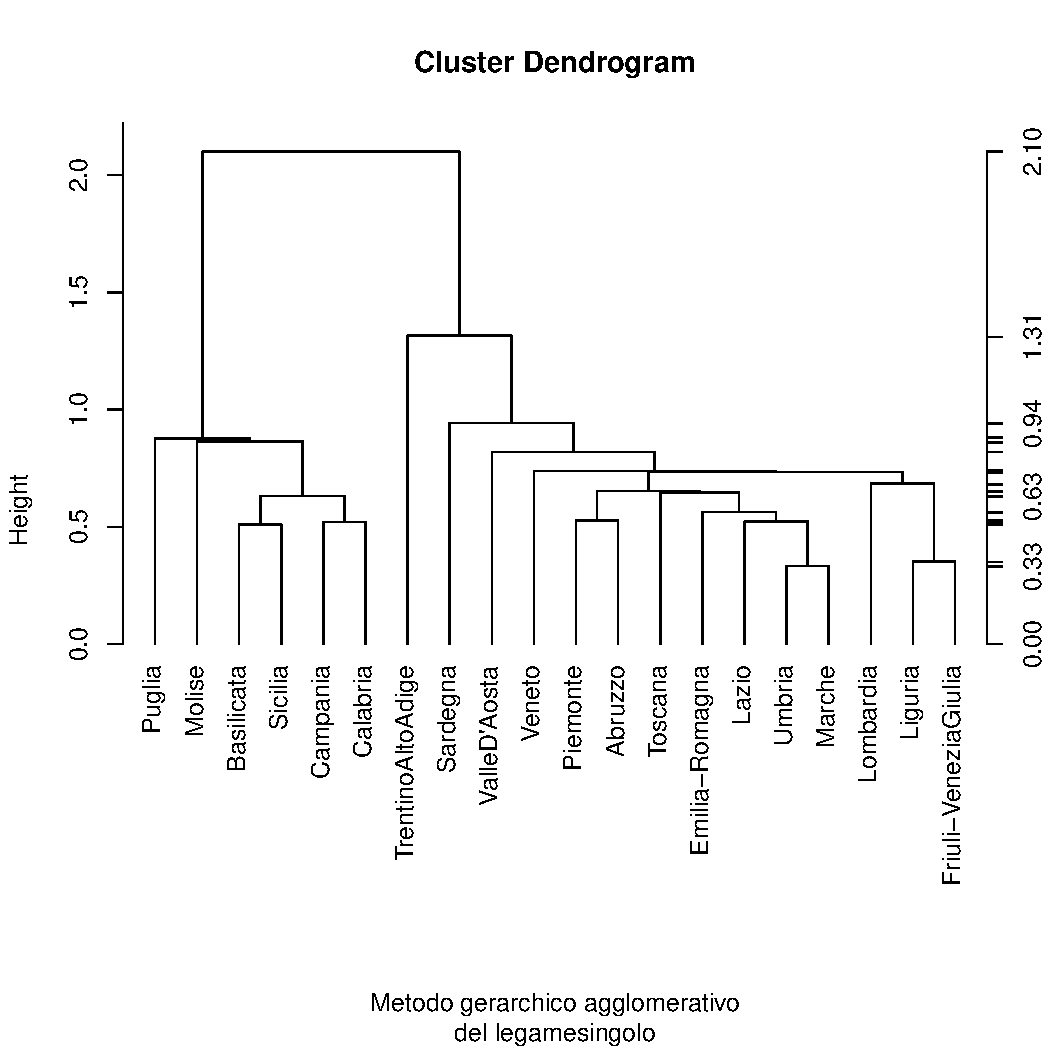
\includegraphics[height=16cm]{ProgettoSAD/capitoli/images/clustering/dendro_cl_singolo.pdf}
\end{figure}
\vspace{5mm}
\newpage

\noindent \textbf{Suddivisione grafica in cluster}

In R la funzione \textit{rect.hclust()} permette di disegnare dei rettangoli intorno ai cluster, evidenziandone la suddivisione.

\vspace{5mm}
\begin{lstlisting}
  rect.hclust(cluster_single, k = 3, border = "green")
\end{lstlisting}
\vspace{5mm}

\vspace{5mm}
\begin{figure}[!htbp]
    \centering
    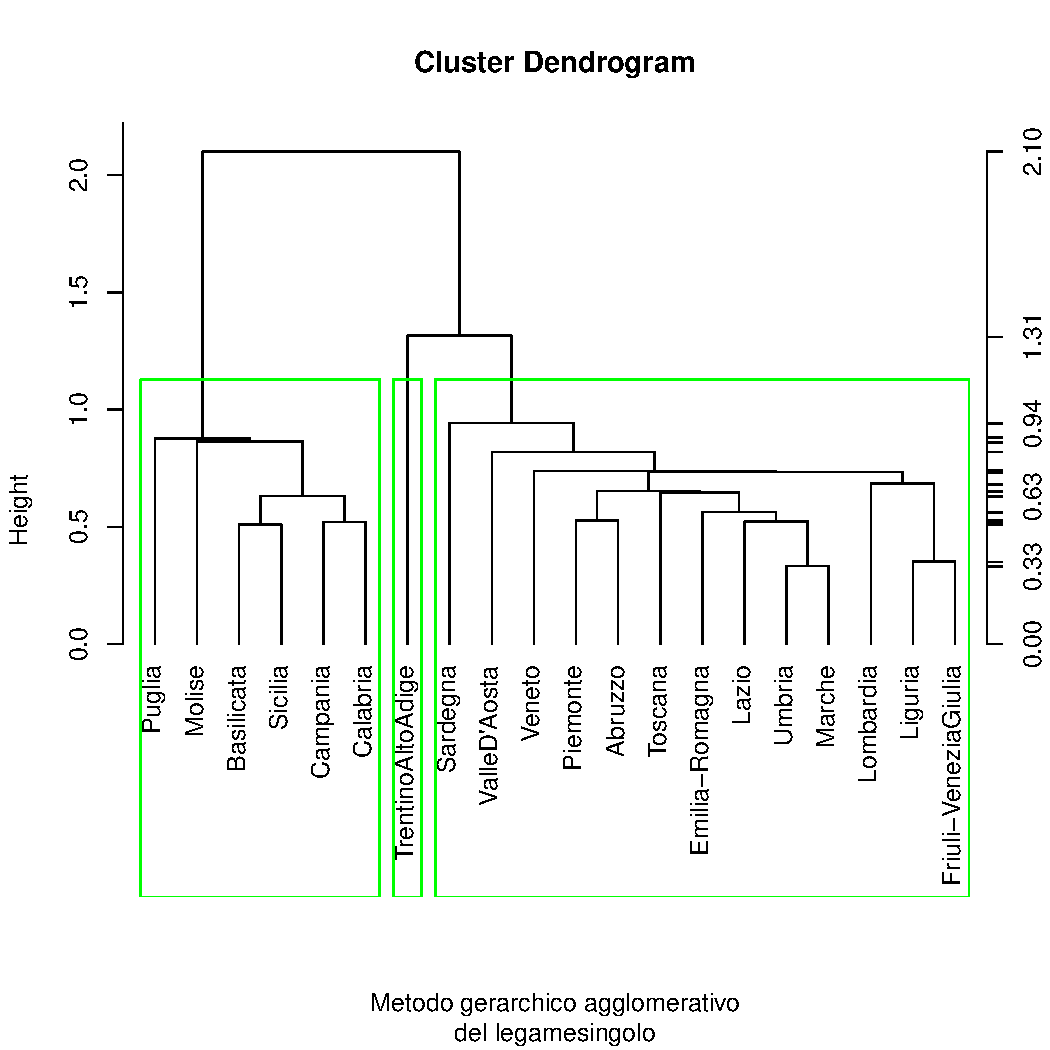
\includegraphics[height=16cm]{ProgettoSAD/capitoli/images/clustering/dendro_cl_sing_sudd.pdf}
\end{figure}
\vspace{5mm}

\noindent \textbf{Individui nei cluster}

In R si utilizza la funzione \textit{cutree()} per evidenziare a quale cluster appartiene ogni individuo.

\vspace{5mm}
\begin{lstlisting}
 cutree(cluster_single, k=3, h=NULL)
 
            Piemonte          ValleDAosta              Liguria 
                   1                    1                    1 
           Lombardia    TrentinoAltoAdige               Veneto 
                   1                    2                    1 
Friuli-VeneziaGiulia       Emilia-Romagna              Toscana 
                   1                    1                    1 
              Umbria               Marche                Lazio 
                   1                    1                    1 
             Abruzzo               Molise             Campania 
                   1                    3                    3 
              Puglia           Basilicata             Calabria 
                   3                    3                    3 
             Sicilia             Sardegna 
                   3                    1 
\end{lstlisting}
\vspace{5mm}

\noindent \textbf{Misure di sintesi associate ai cluster}

È possibile ricavare misure di sintesi (ad esempio la media campionaria, la varianza campionaria, la deviazione standard) sui singoli cluster, ottenuti tagliando il dendrogramma tramite la funzione \textit{cutree()}, utilizzando la funzione \textit{aggregate()}.

\vspace{5mm}
\begin{lstlisting}
  #Misure di sintesi associate ai cluster
  cut_single <- cutree(cluster_single, k = 3)
  cutList_single <- list(cut_single)

  # - Media
  aggregate(df, cutList_single, mean)

  Group.1 Modo.Cont. Modo.Salt. Qualche.Att. Non.Prat.Sport.
1       1   25.91538   12.01538     34.29231        27.73846
2       2   39.80000   14.40000     32.20000        13.50000
3       3   15.83333    8.05000     26.45000        49.68333

  # - Varianza
  aggregate(df, cutList_single, var)

  Group.1 Modo.Cont. Modo.Salt. Qualche.Att. Non.Prat.Sport.
1       1   7.568077    2.43641     5.422436       19.880897
2       2         NA         NA           NA              NA
3       3   1.378667    2.27500     5.027000        6.889667

  # - Devianza standard
  aggregate(df, cutList_single, sd)

  Group.1 Modo.Cont. Modo.Salt. Qualche.Att. Non.Prat.Sport.
1       1   2.751014    1.56090     2.328612        4.458800
2       2         NA         NA           NA              NA
3       3   1.174166    1.50831     2.242097        2.624817
\end{lstlisting}
\vspace{5mm}

Dai risultati ottenuti possiamo notare che alcuni valori sono indicati come NA: questo indica che il cluster contiene un solo individuo, e automaticamente la varianza e la deviazione standard non possono essere calcolate.

\vspace{5mm}
\noindent \textbf{Misure di non omogeneità}

Dopo aver effettuato il taglio, si è interessati a calcolare le misure di non omogeneità statistica relative all'insieme totale di individui (\textit{trT}), ai singoli cluster ottenuti effettuando il taglio e alla somma delle loro misure di non omogeneità (\textit{trS - within}) e alla misura di non omogeneità tra i cluster (\textit{trB - between}):

\[trT = trS + trB\]

Poiché per ogni fissata matrice \textit{X} dei dati si ha che la \textit{trT} è fissata, i cluster dovrebbero essere individuati in modo da minimizzare la misura di non omogeneità statistica all'interno dei cluster (within) e massimizzare la misura di non omogeneità statistica tra i gruppi (between).

\vspace{5mm}
\noindent \textbf{Misura di non omogeneità statistica totale}

\textbf{Definizione:} Si definisce \textit{misura di non omogeneità statistica} dell'insieme I di individui la traccia della matrice $H_I$:

\[trH_i = (n-1) \sum_{r=1}^p s_r^2\]

dove $H_I$ indica la matrice statistica di non omogeneità per l'insieme \textit{I} di individui di cardinalità $p x p$.

La misura di non omogeneità statistica totale può essere così calcolata:

\vspace{5mm}
\begin{lstlisting}
  #Misura di non omogeneità statistica totale
  n <- nrow(df_scaled)
  trH <- (n - 1) * sum(apply(df_scaled, 2, var))
  trH
  [1] 76
\end{lstlisting}
\vspace{5mm}

In R utilizzando la funzione \textit{apply(X, 2, var)} è possibile calcolare la varianza campionaria delle colonne di una matrice.

\vspace{5mm}
\noindent Nota: la misura di non omogeneità totale $trH$ è fissata per il dataset ottenuto, quindi sarà utilizzata anche per i metodi successivi.

\noindent \textbf{Misure di non omogeneità statistiche nei cluster - metodo 2}

Siano $I = I_1, I_2, ..., I_{n1}$ e $J = J_1, J_2, ..., J_{n2}$ due cluster distinti di individui di una popolazione. La misura di non omogeneità statistica tra cluster (\textit{between}) può essere semplicemente calcolata come:

\[trH_{I\cap J} = trH_{I\cup J} - trH_I - trH_j\]

mentre la misura di non omogeneità nei cluster (\textit{within}) può essere semplicemente calcolata come:

\[trH_I + trH_J\]

Tale concetto può essere esteso ai cluster ottenuti precedentemente:

\vspace{5mm}
\begin{lstlisting}
  #Misura di non omogeneità statistica dei tre cluster
  num <- table(cut_single)

  agvar <- aggregate(df_scaled, cutList_single, var)[, -1]

  trH1_single <- (num[[1]] - 1) * sum(agvar[1,])
  trH1_single
  [1] 12.19811

  trH2_single <- (num[[2]] - 1) * sum(agvar[2,])
  trH2_single  
  [1] NA

  trH3_single <- (num[[3]] - 1) * sum(agvar[3,])
  trH3_single
  [1] 3.638836
\end{lstlisting}
\vspace{5mm}

Dalle misure di non omogeneità totale e di non omogeneità nei singoli cluster si ha che:

\[trB = trH - (trH_1 + trH_2 + trH_3) = \]

\[76 - (12.19811 + 0 + 3.638836) = 60,163054\]

\noindent la misura di non omogeneità tra i cluster è più alta rispetto alla misura di non omogeneità all'interno dei cluster($trS$ = 15,836946, la somma dei $trH$), comportando una discreta clusterizzazione.

Effettuando il rapporto

\[60,163054 / 76 = 0,791619 = 79,1\%\]

si ottiene un valore peggiore rispetto all'81.4\% ottenuto con il metodo non gerarchico.

\subsection{Metodo del legame completo}\label{cap5.2.2}

In questo metodo la distanza tra i gruppi $G_1$ (contenente $n_1$ individui) e $G_2$ (contenente $n_2$ individui) è definita come la massima tra tutte le $n_1 n_2$ distanze che si possono calcolare tra ogni individuo di $G_1$ e ogni individuo di $G_2$.

\[d_{(u,v), z} = max(d_{uz}, d_{vz})\]

\noindent \textbf{Clustering tramite il metodo del legame completo}

\vspace{5mm}
\begin{lstlisting}
  cluster_complete <- hclust(dist_e, method = "complete")
  str(cluster_complete)

  List of 7
 $ merge      : int [1:19, 1:2] -10 -3 -17 -15 -1 -12 -8 -4 5 3 ...
 $ height     : num [1:19] 0.334 0.352 0.511 0.52 0.526 ...
 $ order      : int [1:20] 16 14 17 19 15 18 5 20 8 9 ...
 $ labels     : chr [1:20] "Piemonte" "ValleD'Aosta" "Liguria" "Lombardia" ...
 $ method     : chr "complete"
 $ call       : language hclust(d = dist_e, method = "complete")
 $ dist.method: chr "euclidean"
 - attr(*, "class")= chr "hclust"
\end{lstlisting}
\vspace{5mm}

Mostrando l'attributo $\$merge$ si può vedere per intero il processo di clusterizzazione:

\vspace{5mm}
\begin{lstlisting}
 cluster_complete$merge

      [,1] [,2]
 [1,]  -10  -11
 [2,]   -3   -7
 [3,]  -17  -19
 [4,]  -15  -18
 [5,]   -1  -13
 [6,]  -12    1
 [7,]   -8   -9
 [8,]   -4   -6
 [9,]    5    6
[10,]    3    4
[11,]   -2    8
[12,]    7    9
[13,]  -14   10
[14,]  -20   12
[15,]  -16   13
[16,]    2   11
[17,]   14   16
[18,]   -5   17
[19,]   15   18
\end{lstlisting}
\vspace{5mm}

Ad esempio è possibile osservare che sono stati all'inizio raggruppati gli elementi -10 e -11, poi -3 e -7 e così via.

\noindent \textbf{Dendrogramma dei cluster ottenuti}

\vspace{5mm}
\begin{lstlisting}
  plot(cluster_complete, hang = -1, xlab = "Metodo gerarchico
    agglomerativo", sub = "del legame completo")
  axis(side = 4, at = round(c(0, cluster_complete$height), 2))
\end{lstlisting}
\vspace{5mm}

\vspace{5mm}
\begin{figure}[!htbp]
    \centering
    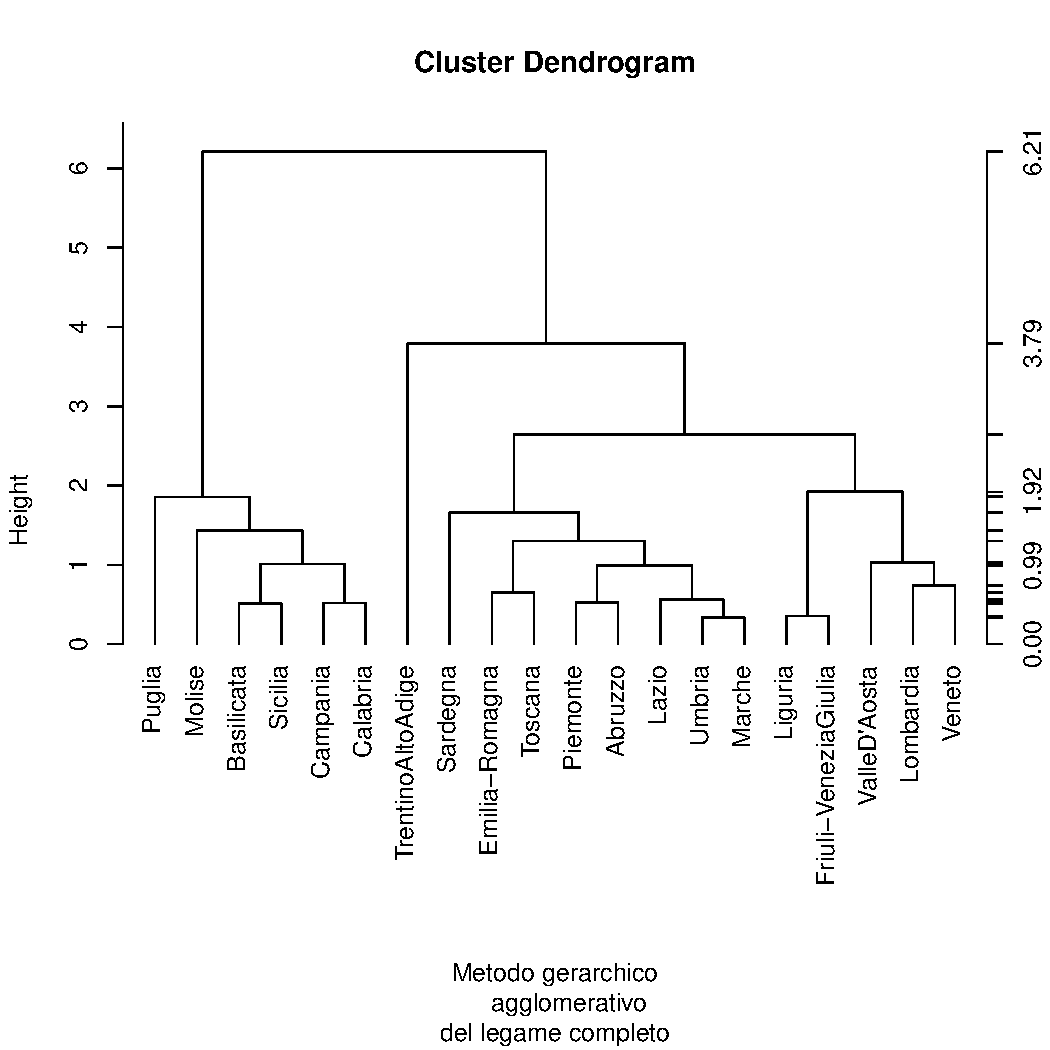
\includegraphics[height=16cm]{ProgettoSAD/capitoli/images/clustering/dendro_clcomp.pdf}
\end{figure}
\vspace{5mm}

\noindent \textbf{Suddivisione grafica in cluster}

\vspace{5mm}
\begin{lstlisting}
rect.hclust(cluster_complete, k = 3, border = "green")
\end{lstlisting}
\vspace{5mm}

\vspace{5mm}
\begin{figure}[!htbp]
    \centering
    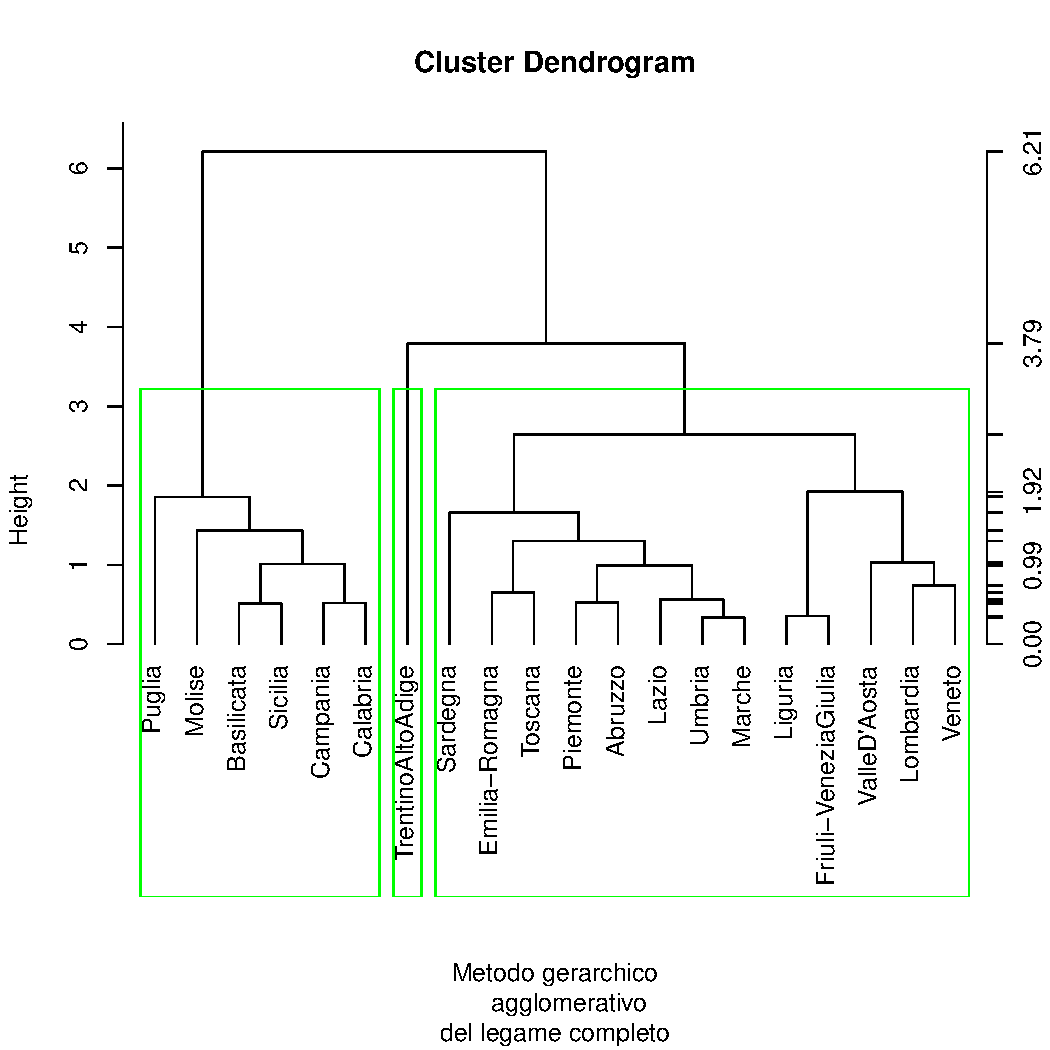
\includegraphics[height=16cm]{ProgettoSAD/capitoli/images/clustering/dendro_clcomp_sudd.pdf}
\end{figure}
\vspace{5mm}

\noindent \textbf{Individui nei cluster}

\vspace{5mm}
\begin{lstlisting}
cutree(cluster_complete, k=3, h=NULL)

            Piemonte          ValleDAosta              Liguria 
                   1                    1                    1 
           Lombardia    TrentinoAltoAdige               Veneto 
                   1                    2                    1 
Friuli-VeneziaGiulia       Emilia-Romagna              Toscana 
                   1                    1                    1 
              Umbria               Marche                Lazio 
                   1                    1                    1 
             Abruzzo               Molise             Campania 
                   1                    3                    3 
              Puglia           Basilicata             Calabria 
                   3                    3                    3 
             Sicilia             Sardegna 
                   3                    1 
\end{lstlisting}
\vspace{5mm}

\noindent \textbf{Misure di sintesi associate ai cluster}

\vspace{5mm}
\begin{lstlisting}
  #Misure di sintesi associate ai cluster
  cut_complete <- cutree(cluster_complete, k = 3)
  cutList_complete <- list(cut_complete)

  # - Media
  aggregate(df, cutList_complete, mean)
  Group.1 Modo.Cont. Modo.Salt. Qualche.Att. Non.Prat.Sport.
1       1   25.91538   12.01538     34.29231        27.73846
2       2   39.80000   14.40000     32.20000        13.50000
3       3   15.83333    8.05000     26.45000        49.68333

  # - Varianza
  aggregate(df, cutList_complete, var)
  
  Group.1 Modo.Cont. Modo.Salt. Qualche.Att. Non.Prat.Sport.
1       1   7.568077    2.43641     5.422436       19.880897
2       2         NA         NA           NA              NA
3       3   1.378667    2.27500     5.027000        6.889667

  # - Devianza standard
  aggregate(df, cutList_complete, sd)

  Group.1 Modo.Cont. Modo.Salt. Qualche.Att. Non.Prat.Sport.
1       1   2.751014    1.56090     2.328612        4.458800
2       2         NA         NA           NA              NA
3       3   1.174166    1.50831     2.242097        2.624817
\end{lstlisting}
\vspace{5mm}

\noindent \textbf{Misure di non omogeneità}

Si ricorda che la misura di non omogeneità statistica totale è $trH = 76$

\noindent \textbf{Misure di non omogeneità statistica nei cluster - metodo 2}

\vspace{5mm}
\begin{lstlisting}
  #Misura di non omogeneità statistica dei tre cluster
  num <- table(cut_complete)

  agvar <- aggregate(df_scaled, cutList_complete, var)[, -1]

  trH1_complete <- (num[[1]] - 1) * sum(agvar[1,])
  trH1_complete
  [1] 12.19811

  trH2_complete <- (num[[2]] - 1) * sum(agvar[2,])
  trH2_complete
  [1] NA

  trH3_complete <- (num[[3]] - 1) * sum(agvar[3,])
  trH3_complete
  [1] 3.638836
\end{lstlisting}
\vspace{5mm}

Dalle misure di non omogeneità totale e non omogeneità nei singoli cluster si ha che

\[trB = trH - (trH_1 + trH_2 + trH_3) = \]

\[76 - (12.19811 + 0 + 3.638836) = 60,163054\]

\noindent la misura di non omogeneità tra i cluster è uguale a quella con il metodo precedente, non comportando alcuna differenza in termini di clusterizzazione.

\subsection{Metodo del legame medio}\label{cap5.2.3}

In questo metodo la distanza tra i gruppi $G_1$ e $G_2$ è definita come la media aritmetica delle distanze tra tutte le coppie di unità che compongono i due gruppi.

\vspace{5mm}
\begin{figure}[!htbp]
    \centering
    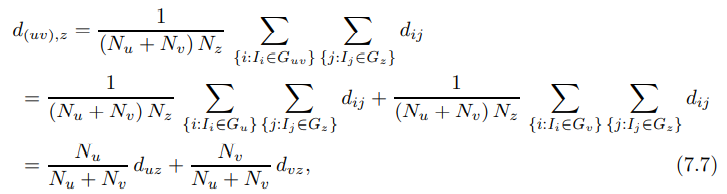
\includegraphics[height=4cm]{ProgettoSAD/capitoli/images/clustering/distanze_legMedio.png}
\end{figure}
\vspace{5mm}

\noindent \textbf{Clustering tramite il metodo del legame medio}

\vspace{5mm}
\begin{lstlisting}
  cluster_average <- hclust(dist_e, method = "average")
  str(cluster_average)

  List of 7
 $ merge      : int [1:19, 1:2] -10 -3 -17 -15 -1 -12 -8 -4 5 3 ...
 $ height     : num [1:19] 0.334 0.352 0.511 0.52 0.526 ...
 $ order      : int [1:20] 16 14 17 19 15 18 5 3 7 2 ...
 $ labels     : chr [1:20] "Piemonte" "ValleD'Aosta" "Liguria" "Lombardia" ...
 $ method     : chr "average"
 $ call       : language hclust(d = dist_e, method = "average")
 $ dist.method: chr "euclidean"
 - attr(*, "class")= chr "hclust"
\end{lstlisting}
\vspace{5mm}

Mostrando l'attributo $\$merge$ si può vedere per intero il processo di clusterizzazione:

\vspace{5mm}
\begin{lstlisting}
cluster_average$merge

      [,1] [,2]
 [1,]  -10  -11
 [2,]   -3   -7
 [3,]  -17  -19
 [4,]  -15  -18
 [5,]   -1  -13
 [6,]  -12    1
 [7,]   -8   -9
 [8,]   -4   -6
 [9,]    5    6
[10,]    3    4
[11,]   -2    8
[12,]    7    9
[13,]  -14   10
[14,]    2   11
[15,]  -20   12
[16,]  -16   13
[17,]   14   15
[18,]   -5   17
[19,]   16   18
\end{lstlisting}
\vspace{5mm}

Ad esempio, è possibile osservare che sono stati all'inizio raggruppati gli elementi -10 e -11, poi -3 e -7 e così via.

\noindent \textbf{Dendrogramma dei cluster ottenuti}

\vspace{5mm}
\begin{lstlisting}
  plot(cluster_average, hang = -1, xlab = "Metodo gerarchico
    agglomerativo", sub = "del legame medio")
  axis(side = 4, at = round(c(0, cluster_average$height), 2))
\end{lstlisting}
\vspace{5mm}

\vspace{5mm}
\begin{figure}[!htbp]
    \centering
    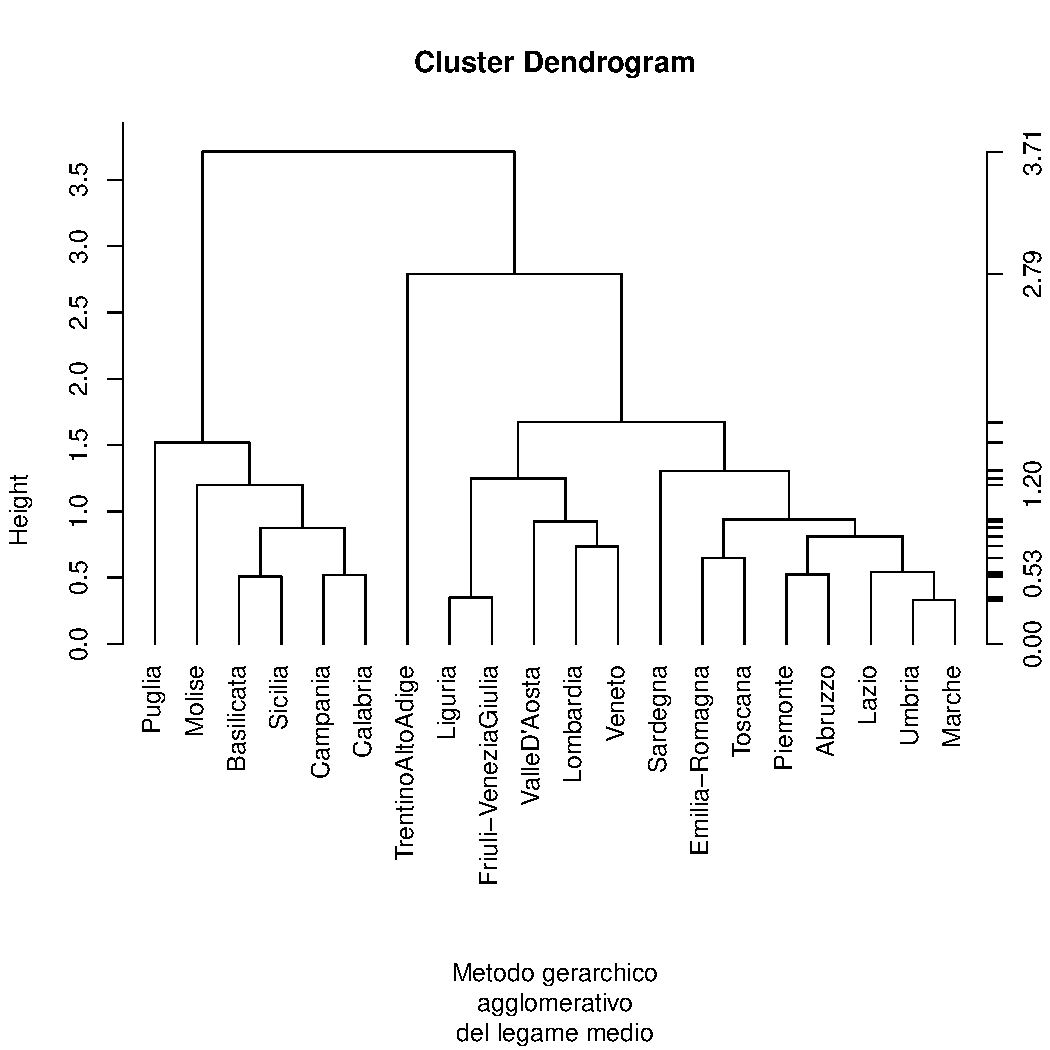
\includegraphics[height=16cm]{ProgettoSAD/capitoli/images/clustering/dendro_cl_medio.pdf}
\end{figure}
\vspace{5mm}

\noindent \textbf{Suddivisione grafica in cluster}

\vspace{5mm}
\begin{lstlisting}
rect.hclust(cluster_average, k = 3, border = "green")
\end{lstlisting}
\vspace{5mm}

\vspace{5mm}
\begin{figure}[!htbp]
    \centering
    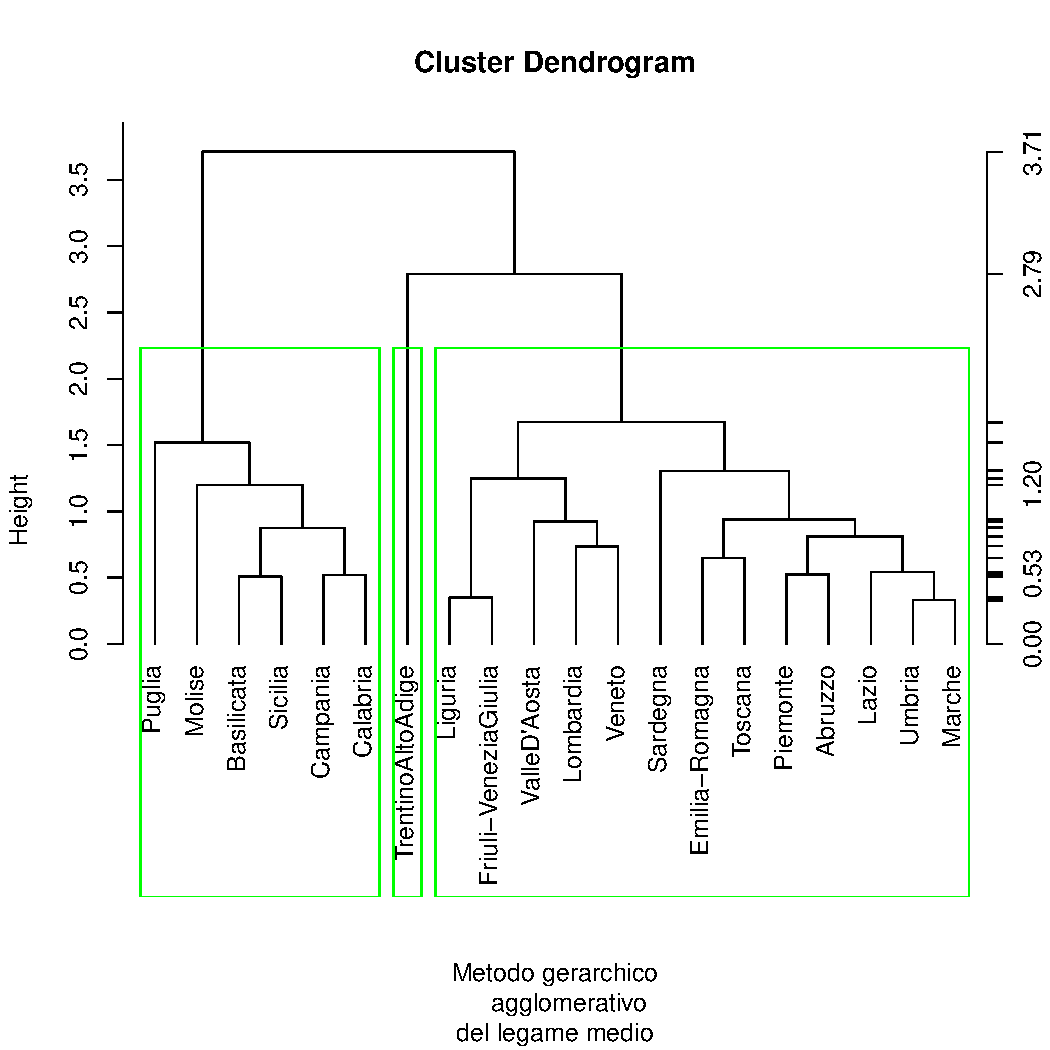
\includegraphics[height=16cm]{ProgettoSAD/capitoli/images/clustering/dendro_cl_medio_sudd.pdf}
\end{figure}
\vspace{5mm}

\noindent \textbf{Individui nei cluster}

\vspace{5mm}
\begin{lstlisting}
cutree(cluster_average, k=3, h=NULL)

            Piemonte          ValleDAosta              Liguria 
                   1                    1                    1 
           Lombardia    TrentinoAltoAdige               Veneto 
                   1                    2                    1 
Friuli-VeneziaGiulia       Emilia-Romagna              Toscana 
                   1                    1                    1 
              Umbria               Marche                Lazio 
                   1                    1                    1 
             Abruzzo               Molise             Campania 
                   1                    3                    3 
              Puglia           Basilicata             Calabria 
                   3                    3                    3 
             Sicilia             Sardegna 
                   3                    1 
\end{lstlisting}
\vspace{5mm}

\noindent \textbf{Misure di sintesi associate ai cluster}

\vspace{5mm}
\begin{lstlisting}
  #Misure di sintesi associate ai cluster
  cut_average <- cutree(cluster_average, k = 3)
  cutList_average <- list(cut_average)

  # - Media
  aggregate(df, cutList_average, mean)

  Group.1 Modo.Cont. Modo.Salt. Qualche.Att. Non.Prat.Sport.
1       1   25.91538   12.01538     34.29231        27.73846
2       2   39.80000   14.40000     32.20000        13.50000
3       3   15.83333    8.05000     26.45000        49.68333

  # - Varianza
  aggregate(df, cutList_average, var)

  Group.1 Modo.Cont. Modo.Salt. Qualche.Att. Non.Prat.Sport.
1       1   7.568077    2.43641     5.422436       19.880897
2       2         NA         NA           NA              NA
3       3   1.378667    2.27500     5.027000        6.889667

  # - Devianza standard
  aggregate(df, cutList_average, sd)

  Group.1 Modo.Cont. Modo.Salt. Qualche.Att. Non.Prat.Sport.
1       1   2.751014    1.56090     2.328612        4.458800
2       2         NA         NA           NA              NA
3       3   1.174166    1.50831     2.242097        2.624817
\end{lstlisting}
\vspace{5mm}

\noindent \textbf{Misure di non omogeneità}

Si ricorda che la misura id non omogeneità statistica totale è $trH = 76$

\noindent \textbf{Misure di non omogeneità statistiche nei cluster - metodo 2}

\vspace{5mm}
\begin{lstlisting}
#Misura di non omogeneità statistica dei tre cluster
  num <- table(cut_average)

  agvar <- aggregate(df_scaled, cutList_average, var)[, -1]

  trH1_average <- (num[[1]] - 1) * sum(agvar[1,])
  trH1_average
  [1] 12.19811

  trH2_average <- (num[[2]] - 1) * sum(agvar[2,])
  trH2_average
  [1] NA

  trH3_average <- (num[[3]] - 1) * sum(agvar[3,])
  trH3_average
  [1] 3.638836
\end{lstlisting}
\vspace{5mm}

Dalle misure di non omogeneità totale e di non omogeneità nei singoli cluster si ha che:

\[trB = trH - (trH_1 + trH_2 + trH_3) = \]

\[76 - (12.19811 + 0 + 3.638836) = 60,163054\]

\noindent la misura di non omogeneità tra i cluster è uguale a quella con il metodo precedente, non comportando alcuna differenza in termini di clusterizzazione.

\subsection{Metodo del centroide}\label{cap5.2.4}

In questo metodo, la distanza tra il gruppo $G_1$ e il gruppo $G_2$ è definita come la distanza tra i centroidi, ossia tra le medie campionarie calcolate sugli individui appartenenti ai due gruppi. Nel metodo del centroide bisogna considerare la distanza al quadrato. Si costruisce, dunque, la matrice contenente i quadrati delle distanze euclidee:

\vspace{5mm}
\begin{lstlisting}
  dist_e2 <- dist_e^2
\end{lstlisting}
\vspace{5mm}

Ad ogni passo successivo, dopoche i cluster $G_1$ e $G_2$ sono stati uniti scegliendo dalla precedente matrice dei quadrati delle distanze euclidee i due cluster più vicini, la distanza tra il nuovocluster, denotato con $G_{uv}$, e un altro cluster $G_z$ è così definita:

\[d_{(u, v), z}^2 = \sum_{k=1}^p(\Bar{x}_{(u, v), k} - \Bar{x}_{(z), k})^2 = \frac{N_u}{N_u + N_v} d_{uz}^2 + \frac{N_v}{N_u + N_v} d_{vz}^2 - \frac{N_uN_v}{(N_u + N_v)^2} d_{u,z}^2\]

dove 

\vspace{5mm}
\begin{figure}[!htbp]
    \centering
    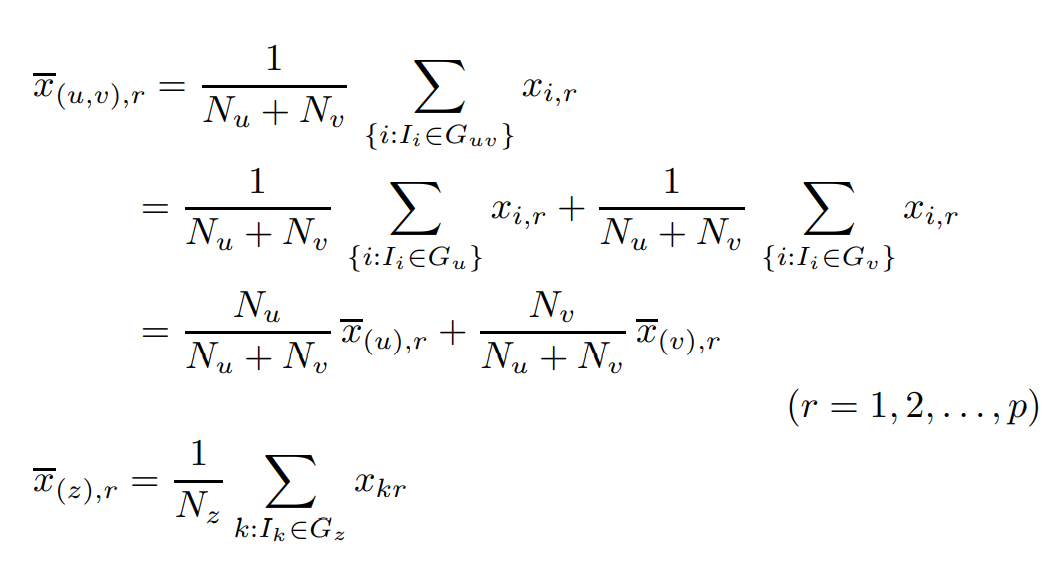
\includegraphics[height=8cm]{ProgettoSAD/capitoli/images/clustering/xuxz.png}
\end{figure}
\vspace{5mm}

\noindent \textbf{Clustering tramite il metodo del centroide}

\vspace{5mm}
\begin{lstlisting}
  cluster_centroid <- hclust(dist_e2, method = "centroid")
  str(cluster_centroid)

  List of 7
 $ merge      : int [1:19, 1:2] -10 -3 -17 -12 -15 -1 -8 4 -4 7 ...
 $ height     : num [1:19] 0.111 0.124 0.261 0.267 0.271 ...
 $ order      : int [1:20] 16 14 17 19 15 18 5 3 7 2 ...
 $ labels     : chr [1:20] "Piemonte" "ValleD'Aosta" "Liguria" "Lombardia" ...
 $ method     : chr "centroid"
 $ call       : language hclust(d = dist_e2, method = "centroid")
 $ dist.method: chr "euclidean"
 - attr(*, "class")= chr "hclust"
\end{lstlisting}
\vspace{5mm}

Mostrando l'attributo $\$merge$ si può osservare per intero il processo di clusterizzazione:

\vspace{5mm}
\begin{lstlisting}
  cluster_centroid$merge

        [,1] [,2]
 [1,]  -10  -11
 [2,]   -3   -7
 [3,]  -17  -19
 [4,]  -12    1
 [5,]  -15  -18
 [6,]   -1  -13
 [7,]   -8   -9
 [8,]    4    6
 [9,]   -4   -6
[10,]    7    8
[11,]    3    5
[12,]   -2    9
[13,]  -14   11
[14,]    2   12
[15,]  -20   10
[16,]   14   15
[17,]  -16   13
[18,]   -5   16
[19,]   17   18
\end{lstlisting}
\vspace{5mm}

Ad esempio è possibile osservare che all'inizio sono stati raggruppati gli individui -5 e -16, poi gli individui -1 e -4 e così via.

\textbf{Dendrogramma dei cluster ottenuti}

\vspace{5mm}
\begin{lstlisting}
  plot(cluster_centroid, hang = -1, xlab = "Metodo gerarchico
    agglomerativo", sub = "del centroide")
  axis(side = 4, at = round(c(0, cluster_centroid$height), 2))
\end{lstlisting}
\vspace{5mm}

\vspace{5mm}
\begin{figure}[!htbp]
    \centering
    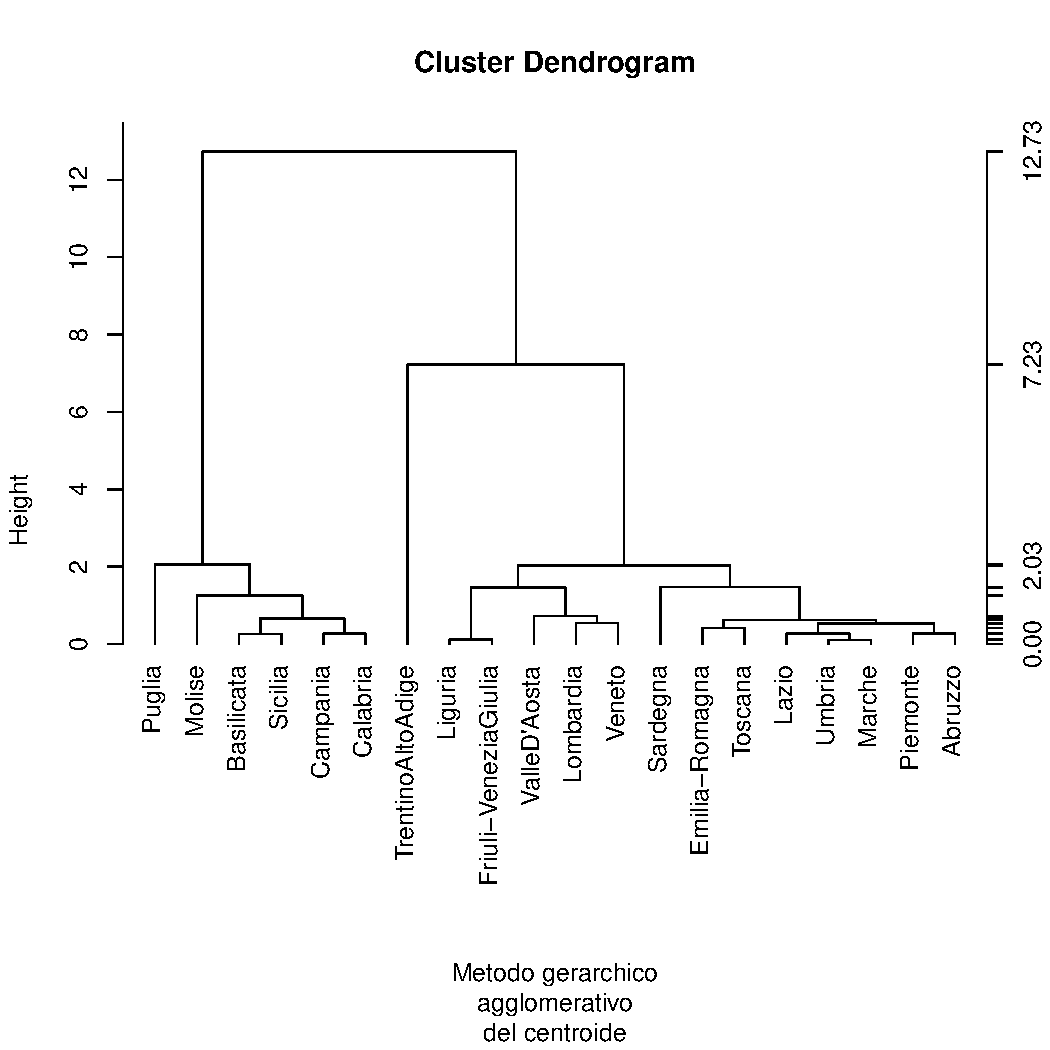
\includegraphics[height=16cm]{ProgettoSAD/capitoli/images/clustering/dendro_clcentr.pdf}
\end{figure}
\vspace{5mm}

\noindent \textbf{Suddivisione grafica in cluster}

\vspace{5mm}
\begin{lstlisting}
rect.hclust(cluster_centroid, k = 3, border = "green")
\end{lstlisting}
\vspace{5mm}

\vspace{5mm}
\begin{figure}[!htbp]
    \centering
    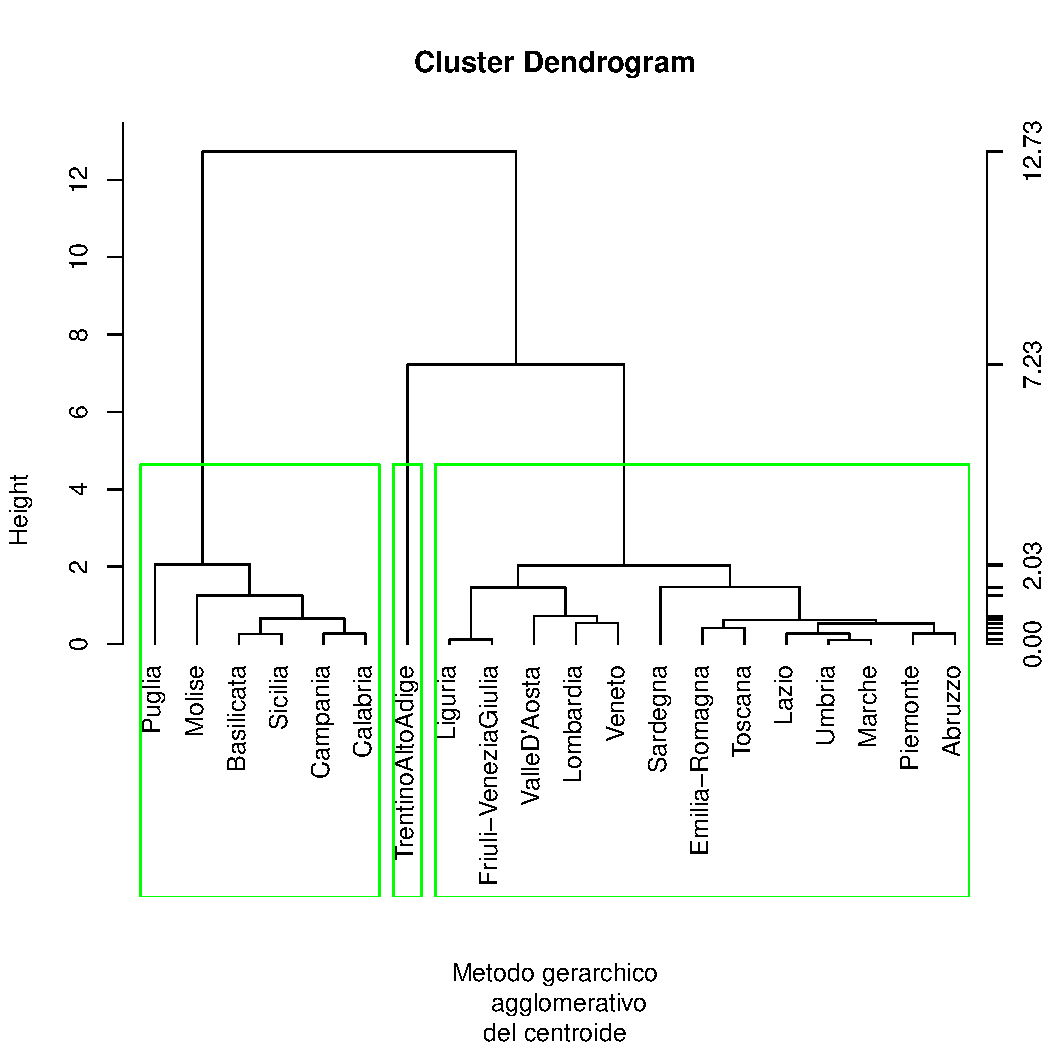
\includegraphics[height=16cm]{ProgettoSAD/capitoli/images/clustering/dendro_clcentr_sudd.pdf}
\end{figure}
\vspace{5mm}

\noindent \textbf{Individui nei cluster}

\vspace{5mm}
\begin{lstlisting}
cutree(cluster_centroid, k=5, h=NULL)

            Piemonte          ValleDAosta              Liguria 
                   1                    1                    1 
           Lombardia    TrentinoAltoAdige               Veneto 
                   1                    2                    1 
Friuli-VeneziaGiulia       Emilia-Romagna              Toscana 
                   1                    1                    1 
              Umbria               Marche                Lazio 
                   1                    1                    1 
             Abruzzo               Molise             Campania 
                   1                    3                    3 
              Puglia           Basilicata             Calabria 
                   3                    3                    3 
             Sicilia             Sardegna 
                   3                    1 
\end{lstlisting}
\vspace{5mm}

\noindent \textbf{Misure di sintesi associate ai cluster}

\vspace{5mm}
\begin{lstlisting}
  #Misure di sintesi associate ai cluster
  cut_centroid <- cutree(cluster_centroid, k = 3)
  cutList_centroid <- list(cut_centroid)

  # - Media
  aggregate(df, cutList_centroid, mean)

  Group.1 Modo.Cont. Modo.Salt. Qualche.Att. Non.Prat.Sport.
1       1   25.91538   12.01538     34.29231        27.73846
2       2   39.80000   14.40000     32.20000        13.50000
3       3   15.83333    8.05000     26.45000        49.68333

  # - Varianza
  aggregate(df, cutList_centroid, var

  Group.1 Modo.Cont. Modo.Salt. Qualche.Att. Non.Prat.Sport.
1       1   7.568077    2.43641     5.422436       19.880897
2       2         NA         NA           NA              NA
3       3   1.378667    2.27500     5.027000        6.889667

  # - Devianza standard
  aggregate(df, cutList_centroid, sd)

  Group.1 Modo.Cont. Modo.Salt. Qualche.Att. Non.Prat.Sport.
1       1   2.751014    1.56090     2.328612        4.458800
2       2         NA         NA           NA              NA
3       3   1.174166    1.50831     2.242097        2.624817
\end{lstlisting}
\vspace{5mm}

\noindent \textbf{Misure di non omogeneità}

Si ricorda che la misura id non omogeneità statistica totale è $trH = 76$

\noindent \textbf{Misure di non omogeneità statistiche nei cluster - metodo 2}

\vspace{5mm}
\begin{lstlisting}
  #Misura di non omogeneità statistica dei tre cluster
  num <- table(cut_centroid)

  agvar <- aggregate(df_scaled, cutList_centroid, var)[, -1]

  trH1_centroid <- (num[[1]] - 1) * sum(agvar[1,])
  trH1_centroid
  [1] 12.19811

  trH2_centroid <- (num[[2]] - 1) * sum(agvar[2,])
  trH2_centroid
  [1] NA

  trH3_centroid <- (num[[3]] - 1) * sum(agvar[3,])
  trH3_centroid
  [1] 3.638836
\end{lstlisting}
\vspace{5mm}

Dalle misure di non omogeneità totale e di non omogeneità nei singoli cluster si ha che

\[trB = trH - (trH_1 + trH_2 + trH_3) = \]

\[76 - (12.19811 + 0 + 3.638836) = 60,163054\]

\noindent la misura di non omogeneità tra i cluster è quasi uguale a quelle considerando il legame completo e il legame medio, quindi vale lo stesso discorso fatto in precedenza. 

\subsection{Metodo della mediana}\label{cap5.2.5}

Il metodo della mediana è simile a quello del centroide, con la differenza che la procedura è indipendente dalla numerosità dei cluster. Infatti, quando due gruppi si aggregano, il nuovo centroide è calcolato come la semisomma dei due centroidi precedenti. Anche in questo caso va considerata la distanza al quadrato. Ad ogni passo successivo, dopo che i cluster $G_1$ e $G_2$ sono stati uniti scegliendo dalla precedente matrice dei quadrati delle distanze euclidee i due cluster più vicini, la distanza tra il nuovo cluster  $G_{uv}$, e un altro cluster $G_z$ è così definita:

\[d_{(uv),z}^2 = \sum_{k=1}^p(\Bar{x}_{(u,v),k} - \Bar{x}_{(z), k})^2 = \frac{1}{2}d_{u,z}^2 + \frac{1}{2}d_{v,z}^2 - \frac{1}{4}d_{u,v}^2\]

\noindent \textbf{Clustering tramite il metodo della mediana}

\vspace{5mm}
\begin{lstlisting}
  cluster_median <- hclust(dist_e2, method = "median")
  str(cluster_median)

  List of 7
 $ merge      : int [1:19, 1:2] -10 -3 -17 -12 -15 -1 -8 -4 4 3 ...
 $ height     : num [1:19] 0.111 0.124 0.261 0.267 0.271 ...
 $ order      : int [1:20] 16 14 17 19 15 18 5 20 8 9 ...
 $ labels     : chr [1:20] "Piemonte" "ValleD'Aosta" "Liguria" "Lombardia" ...
 $ method     : chr "median"
 $ call       : language hclust(d = dist_e2, method = "median")
 $ dist.method: chr "euclidean"
 - attr(*, "class")= chr "hclust"
\end{lstlisting}
\vspace{5mm}

Mostrando l'attributo $\$merge$ si può osservare per intero il processo di clusterizzazione:

\vspace{5mm}
\begin{lstlisting}
cluster_median$merge

      [,1] [,2]
 [1,]  -10  -11
 [2,]   -3   -7
 [3,]  -17  -19
 [4,]  -12    1
 [5,]  -15  -18
 [6,]   -1  -13
 [7,]   -8   -9
 [8,]   -4   -6
 [9,]    4    6
[10,]    3    5
[11,]    7    9
[12,]   -2    8
[13,]  -14   10
[14,]  -20   11
[15,]    2   12
[16,]   14   15
[17,]  -16   13
[18,]   -5   16
[19,]   17   18
\end{lstlisting}
\vspace{5mm}

\noindent \textbf{Dendrogramma dei cluster ottenuti}

\vspace{5mm}
\begin{lstlisting}
  plot(cluster_median, hang = -1, xlab = "Metodo gerarchico agglomerativo", sub = "della
    mediana")
  axis(side = 4, at = round(c(0, cluster_median$height), 2))
\end{lstlisting}
\vspace{5mm}

\vspace{5mm}
\begin{figure}[!htbp]
    \centering
    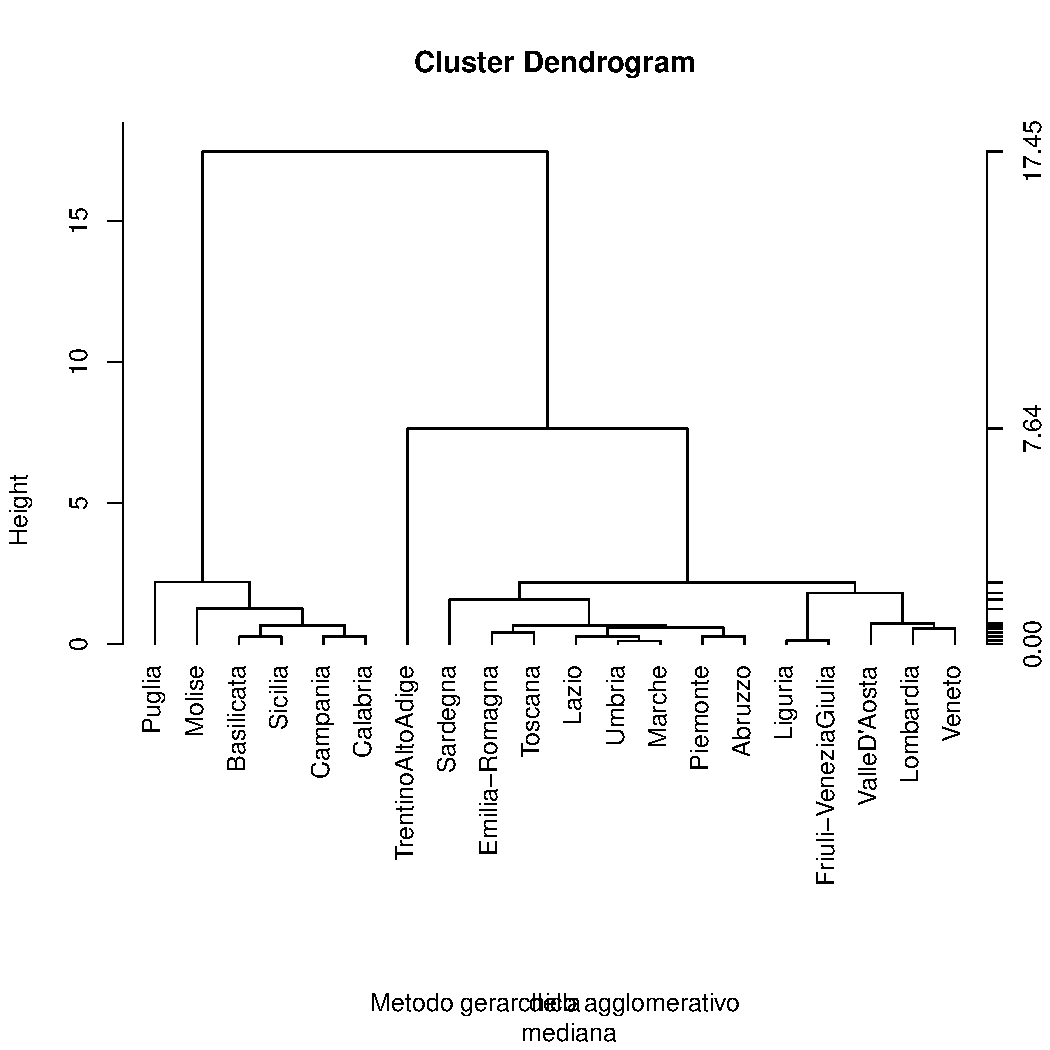
\includegraphics[height=16cm]{ProgettoSAD/capitoli/images/clustering/dendro_clmediana.pdf}
\end{figure}
\vspace{5mm}

\noindent \textbf{Suddivisione grafica in cluster}

\vspace{5mm}
\begin{lstlisting}
rect.hclust(cluster_median, k = 3, border = "green")
\end{lstlisting}
\vspace{5mm}

\vspace{5mm}
\begin{figure}[!htbp]
    \centering
    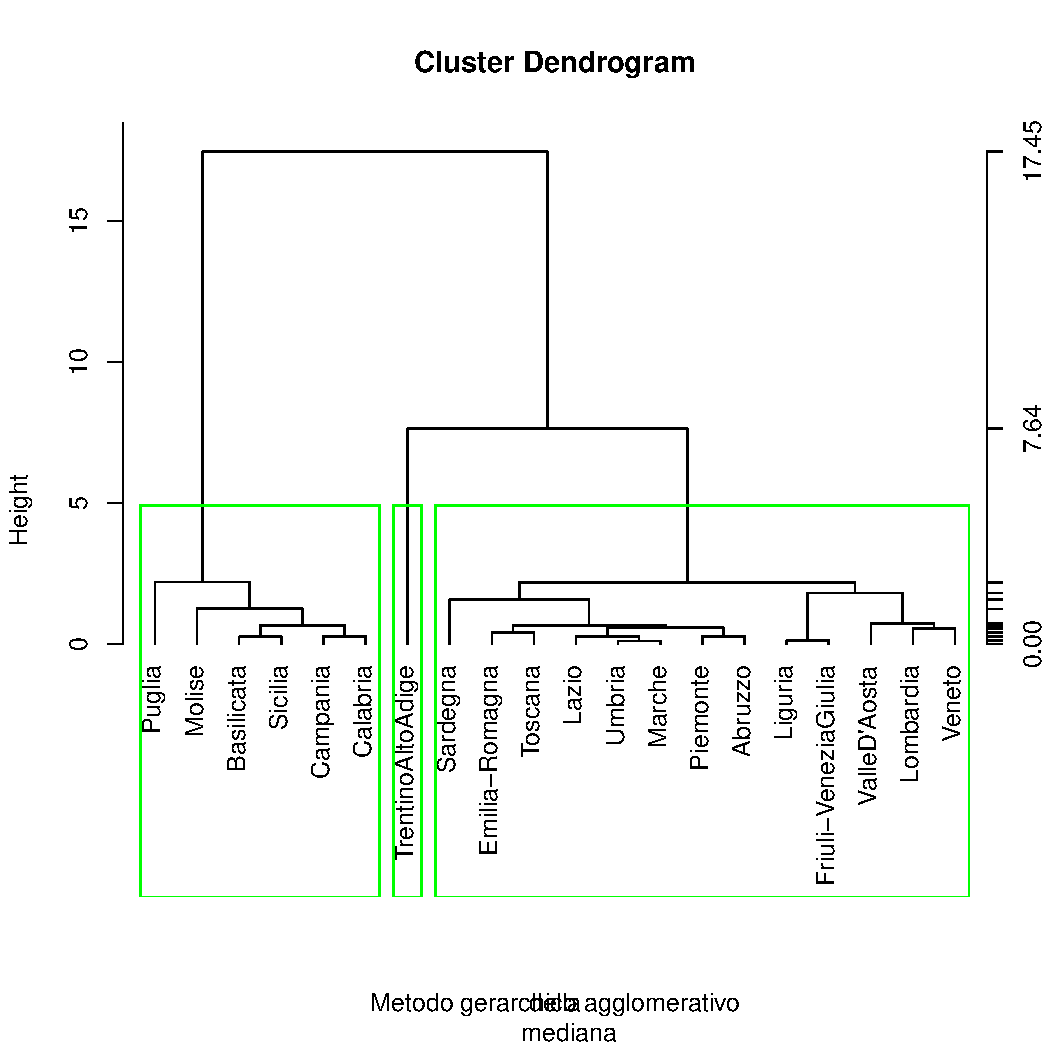
\includegraphics[height=16cm]{ProgettoSAD/capitoli/images/clustering/dendro_clmediana_sudd.pdf}
\end{figure}
\vspace{5mm}

\noindent \textbf{Individui nei cluster}

\vspace{5mm}
\begin{lstlisting}
cutree(cluster_median, k=3, h=NULL)

            Piemonte          ValleDAosta              Liguria 
                   1                    1                    1 
           Lombardia    TrentinoAltoAdige               Veneto 
                   1                    2                    1 
Friuli-VeneziaGiulia       Emilia-Romagna              Toscana 
                   1                    1                    1 
              Umbria               Marche                Lazio 
                   1                    1                    1 
             Abruzzo               Molise             Campania 
                   1                    3                    3 
              Puglia           Basilicata             Calabria 
                   3                    3                    3 
             Sicilia             Sardegna 
                   3                    1 
\end{lstlisting}
\vspace{5mm}

\noindent \textbf{Misure di sintesi associate ai cluster}

\vspace{5mm}
\begin{lstlisting}
  #Misure di sintesi associate ai cluster
  cut_median <- cutree(cluster_median, k = 3)
  cutList_median <- list(cut_median)

  # - Media
  aggregate(df, cutList_median, mean)

  # - Media
  aggregate(df, cutList_centroid, mean)

  Group.1 Modo.Cont. Modo.Salt. Qualche.Att. Non.Prat.Sport.
1       1   25.91538   12.01538     34.29231        27.73846
2       2   39.80000   14.40000     32.20000        13.50000
3       3   15.83333    8.05000     26.45000        49.68333

  # - Varianza
  aggregate(df, cutList_centroid, var

  Group.1 Modo.Cont. Modo.Salt. Qualche.Att. Non.Prat.Sport.
1       1   7.568077    2.43641     5.422436       19.880897
2       2         NA         NA           NA              NA
3       3   1.378667    2.27500     5.027000        6.889667

  # - Devianza standard
  aggregate(df, cutList_centroid, sd)

  Group.1 Modo.Cont. Modo.Salt. Qualche.Att. Non.Prat.Sport.
1       1   2.751014    1.56090     2.328612        4.458800
2       2         NA         NA           NA              NA
3       3   1.174166    1.50831     2.242097        2.624817
\end{lstlisting}
\vspace{5mm}

\noindent \textbf{Misure di non omogeneità}

Si ricorda che la misura id non omogeneità statistica totale è $trH = 76$

\noindent \textbf{Misure di non omogeneità statistiche nei cluster - metodo 2}

\vspace{5mm}
\begin{lstlisting}
  #Misura di non omogeneità statistica dei tre cluster
  num <- table(cut_median)

  agvar <- aggregate(df_scaled, cutList_median, var)[, -1]

  trH1_centroid <- (num[[1]] - 1) * sum(agvar[1,])
  trH1_centroid
  [1] 12.19811

  trH2_centroid <- (num[[2]] - 1) * sum(agvar[2,])
  trH2_centroid
  [1] NA

  trH3_centroid <- (num[[3]] - 1) * sum(agvar[3,])
  trH3_centroid
  [1] 3.638836

\end{lstlisting}
\vspace{5mm}

Dalle misure di non omogeneità totale e non omogeneità nei singoli cluster si ha che

\[trB = trH - (trH_1 + trH_2 + trH_3) = \]

\[76 - (12.19811 + 0 + 3.638836) = 60,163054\]

\noindent la misura di non omogeneità tra i cluster è uguale a quella del metodo precedente del centroide e alle altre, dunque vale lo stesso discorso.

%################################################

\newpage